\section{Passages and loops in the full attractor}\label{sec:loops}
Throughout this section $h\in I_h$. Homology means integral \emph{singular}
homology. A loop is a continuous map from the circle and need not be an
embedded polygon or a smooth curve. We use winding and linking homomorphisms
on the complement of a line or a polygonal wire; these are defined for
arbitrary continuous loops and depend only on their homology classes.

\subsection{A central passage and its winding loop}
\begin{proposition}\label{prop:central}
The closed vertical cylinder of radius $0.0122$ is disjoint from $K$.
There is a loop $\gamma$ in $K$ with winding number one about its axis.
\end{proposition}
\begin{proof}
In the depth-eight grid calculation restricted to $G_0(K)$, the minimum
integer $x$-coordinate is $3,049,454$ and the minimum squared horizontal
radius is $97,951,509,407,090$. Put
$\epsilon=0.00055+2.14(0.476186)^8$. Every attractor point in this piece is
within $\epsilon$ of an appropriate grid centre. Since each centre has
positive $x$, its distance to the half-plane
$H=\{(x,0,z):x\le0\}$ equals its horizontal radius. The exact squared-distance
test proves that its distance to $H$, after subtracting $\epsilon$, exceeds
$0.0122$. Symmetry under $T$ proves cylinder avoidance for all pieces.

The adjacent contact points $T^{-1}p,p$ belong to $G_0(K)$ and lie at
azimuths $-\pi/6,\pi/6$. Their positive radial coordinates are certified by
the contact enclosures. Join them by a path in $G_0(K)$, using path
connectedness. Avoidance of $H$ permits a continuous principal argument
along the path, with total change $\pi/3$. Concatenating its six images
under $T^j$, $0\le j<6$, yields a closed loop with total argument change
$2\pi$. Projection to the circle gives a homomorphism detecting its
nonzero homology class in the full $K$.
\end{proof}

\subsection{Two smaller passages and independent classes}
Define parallel lines, oriented by $d=(-1,0,1)/\sqrt2$, by
\begin{equation}\label{eq:axes}
\ell_\pm=\{(x,0,z):x+z=\pm(1+h)\}.
\end{equation}
Let $\gamma_A=G_0\gamma$ and $\gamma_B=G_3\gamma$.
\begin{proposition}\label{prop:two}
For each sign, $0.105<\dist(K,\ell_\pm)<0.118$. With consistent orientations,
the winding numbers of $\gamma_A,\gamma_B$ about these lines form the identity
matrix. Thus $[\gamma_A],[\gamma_B]$ are linearly independent in $H_1(K;\Z)$.
\end{proposition}
\begin{proof}[Certificate and winding argument]
For sign $s=\pm1$, perpendicular coordinates are
$(X/\sqrt2,Y)$, with $X=x+z-s(1+h)$ and $Y=y$.
The verifier evaluates
\[
(i+k-sQ(1+\widehat h))^2+2j^2
\]
at all grid centres $(i,j,k)$, where
$\widehat h=\lfloor0.7071Q\rfloor/Q$. This is twice the squared physical
line distance after division by $Q^2$. The grid, height and cylinder-tail
allowances give a total distance error less than $0.00631$.
The resulting interval is contained in $(0.105,0.118)$ for both lines.

For each of the six subpieces of the relevant child, the verifier also
certifies a half-plane inequality
\[
\frac{aX+bY}{\sqrt{2a^2+b^2}}>0.06,
\quad (a,b)\in\{(1,0),(-1,2),(1,2),(-1,0),(1,-2),(-1,-2)\},
\]
with the listed normals assigned to the six successive subpieces.
Each projected path segment may therefore be homotoped to its endpoint
chord without crossing the projected origin. The resulting contact hexagon
has winding one: the map on the contact plane for the upper child has
matrix $\operatorname{diag}(r(\cos\alpha-\sin\alpha)/\sqrt2,r)$, with
positive determinant. Symmetry supplies the lower child.
Each child is contained in a ball of radius $2.14r$ clearing the other line
by more than $1.39$, so the two cross-windings vanish. The two winding
homomorphisms read off the coefficients in any relation between the classes.
\end{proof}

\begin{figure}[tb]
\centering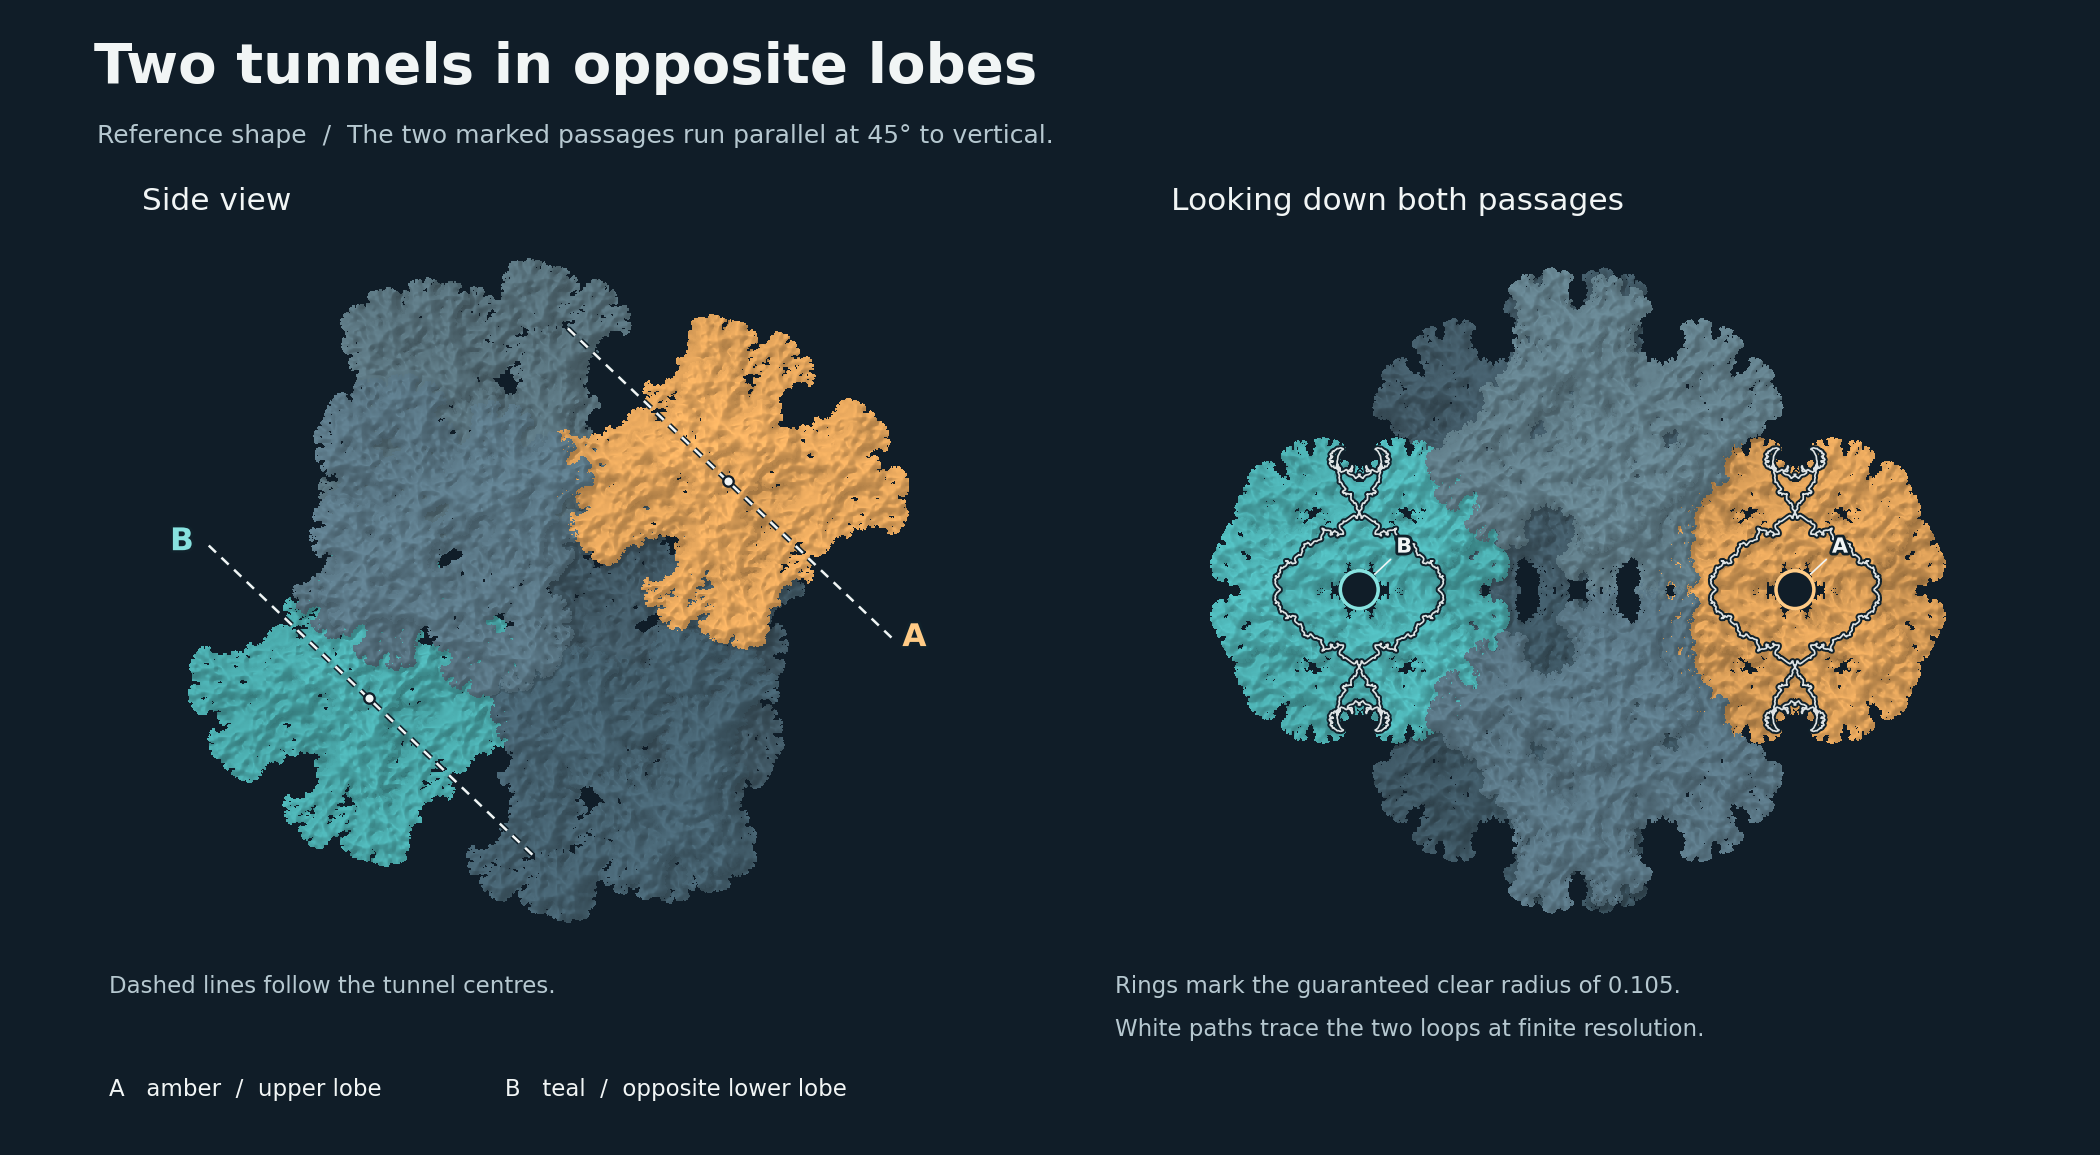
\includegraphics[width=\linewidth]{../research/fractal_research_09/opposite_tunnels.png}
\caption{The two clear lines~\eqref{eq:axes}, with the upper and opposite lower
lobes marked A and B. The rings show a guaranteed clear radius $0.105$;
the drawn paths are finite approximations to the loops used in the argument.
The line directions differ from the original inherited tilted axes discussed
in Section~\ref{sec:bore}.}
\label{fig:two}
\end{figure}

\subsection{Detecting wires at every scale}
The essential question for a repeated loop is whether a neighbouring piece
could fill it in the full attractor. The following construction supplies
detecting curves that avoid \emph{all} pieces.

\begin{theorem}\label{thm:homology}
For every $h\in I_h$ there are countably many linearly independent classes
in $H_1(K(h);\Z)$ represented by loops shrinking to the fixed point $p_*$
of $G_0$. There is a surjective homomorphism
\begin{equation}\label{eq:product}
H_1(K(h);\Z)\longrightarrow\prod_{m\ge0}\Z.
\end{equation}
In particular this homology group is uncountable. At each of the six
symmetry-related fixed points there are arbitrarily small loops that remain
noncontractible in the entire attractor.
\end{theorem}

\begin{proof}
The point $p_*=(I-rQ_0)^{-1}t_0$ is distinct from the periodic contact $p$;
at the reference it is approximately $(1.88117,0,0.44205)$. Set
\[
t=(1,0,h),\quad e=(1,0,1)/\sqrt2,\quad d=(-1,0,1)/\sqrt2,
\quad a=1.03,
\]
and let $D$ be the boundary of the rectangle
\[
\{t+ve+wd:0\le v\le a,\ |w|\le a\}.
\]
Its edge $v=0$ lies on $\ell_+$, which is clear of $K$.
The other three edges are outside $B(t,2.14r)$, since $a>2.14r$.
All sibling enclosing balls lie strictly in $e\cdot(x-t)<0$, so the full
wire misses $K$. Orient $D$ so that its edge on $\ell_+$ follows $d$.
Then $\lk(\gamma_A,D)=1$. Indeed, compactify the line in $S^3$ and replace
its exterior arc by the three remaining rectangle edges. Both arcs lie
outside the child ball and are homotopic relative to endpoints there,
because the exterior of a ball in $S^3$ is simply connected.

The following four strict bounds are interval-certified over the whole family:
\begin{equation}\label{eq:wires}
\begin{split}
\dist\left(p_*,\bigcup_{k\ne0}G_k(K)\right)&>0.96,\\
G_0(D)&\subset B(p_*,0.95),\\
\dist(p_*,D)&>0.19,\\
G_0^4(G_0(K))&\subset B(p_*,0.11).
\end{split}
\end{equation}
The second bound follows from the four rectangle corners and convexity of
the ball. As $G_0$ fixes $p_*$ and contracts, all its later wire images
remain within $B(p_*,0.95)$. Inductively, $G_0^j(D)$ avoids $G_0(K)$ by
injectivity if $G_0^{j-1}(D)$ avoids $K$, and it avoids the siblings by
the first bound. Thus every wire image misses the entire attractor.

For $n,m\ge0$ put
\[
\gamma_n=G_0^{4n}(\gamma_A),\qquad D_m=G_0^{4m}(D).
\]
Similarity invariance gives $\lk(\gamma_m,D_m)=1$. For $n>m$, apply
$G_0^{-4m}$ and use~\eqref{eq:wires}: the smaller loop lies in
$B(p_*,0.11)$, disjoint from $D$. Hence
\begin{equation}\label{eq:triangular}
\lk(\gamma_n,D_m)=
\begin{cases}1,&n=m,\\0,&n>m.\end{cases}
\end{equation}
No assertion is made about entries with $n<m$. Pairing a finite relation
against the wire at its smallest index reads off that coefficient.
Induction gives linear independence.

For the stronger assertion, base $\gamma_A$ at $p_*$ by an out-and-back path
inside $G_0(K)$ and call the resulting loop $\beta_0$.
Set $\beta_n=G_0^{4n}\beta_0$. The connecting paths add no linking number.
For any target integer sequence $(b_m)_{m\ge0}$, recursively choose
\[
c_m=b_m-\sum_{n<m}c_n\lk(\beta_n,D_m).
\]
Concatenate $\beta_m^{c_m}$ on successive time intervals of lengths
$2^{-m-1}$ and end at $p_*$. Each $c_m$ is finite, although the sequence
may be unbounded. The diameters of the based loops tend to zero, so the
infinite concatenation is continuous at its endpoint.
For any fixed $m$, the entire tail after stage $m$ lies in
$B(p_*,0.11r^{4m})$, disjoint from $D_m$ by~\eqref{eq:wires}.
That tail is null-homologous in the wire complement. The resulting loop
therefore has linking record exactly $(b_m)$, proving surjectivity.
The product is uncountable. Finally, symmetry transports the shrinking
essential loops to the other five fixed points.
\end{proof}

This is a quotient statement, not an identification of $H_1(K;\Z)$ with
the product. It does not classify the fundamental group or establish a
homeomorphism with the Hawaiian earring. Infinite concatenations of shrinking
loops are classical \cite[Example 1.25]{hatcher}; the geometry in
\eqref{eq:wires} is what validates their use in this overlapping spatial set.

\subsection{The original tilted bore: obstruction at positive radius}\label{sec:bore}
The original upper child's inherited central axis is the line through
$t=(1,0,h)$ with unit direction $v=(\sin\alpha,0,\cos\alpha)$.
For a point $P=(x,y,z)$ define inward travel and perpendicular distance by
\[
T(P)=-v\cdot(P-t),\qquad
D(P)^2=[\cos\alpha(x-1)-\sin\alpha(z-h)]^2+y^2.
\]
For bore radius $0.0058$, the first intrusion is
$\min\{T(P):P\in K,\ D(P)\le0.0058\}$.
The certificate encloses it in $[1.325115,1.325120]$ at the reference and
in $[1.320,1.330]$ uniformly on the family. Lobes 1 and 5 intrude in the
upper bore; central inversion gives lobes 4 and 2 for the lower bore.
At the reference, the first occupied axis cross-section is near
$(0.33814,0,-0.44088)$.

An actual point with address $1404022400020420424\,0^\infty$ is inside the
reference bore, near $(0.340917,0.004592,-0.442484)$. Its mirror supplies
the other intrusion. This proves nonemptiness of the compact minimisation
set. The lower travel bound follows by discarding word balls from
\eqref{eq:tail} that lie outside the bore or beyond the proposed threshold;
all remaining reference branches close by depth 16. A separate addressed
witness supplies the uniform upper bound.

\begin{figure}[tb]
\centering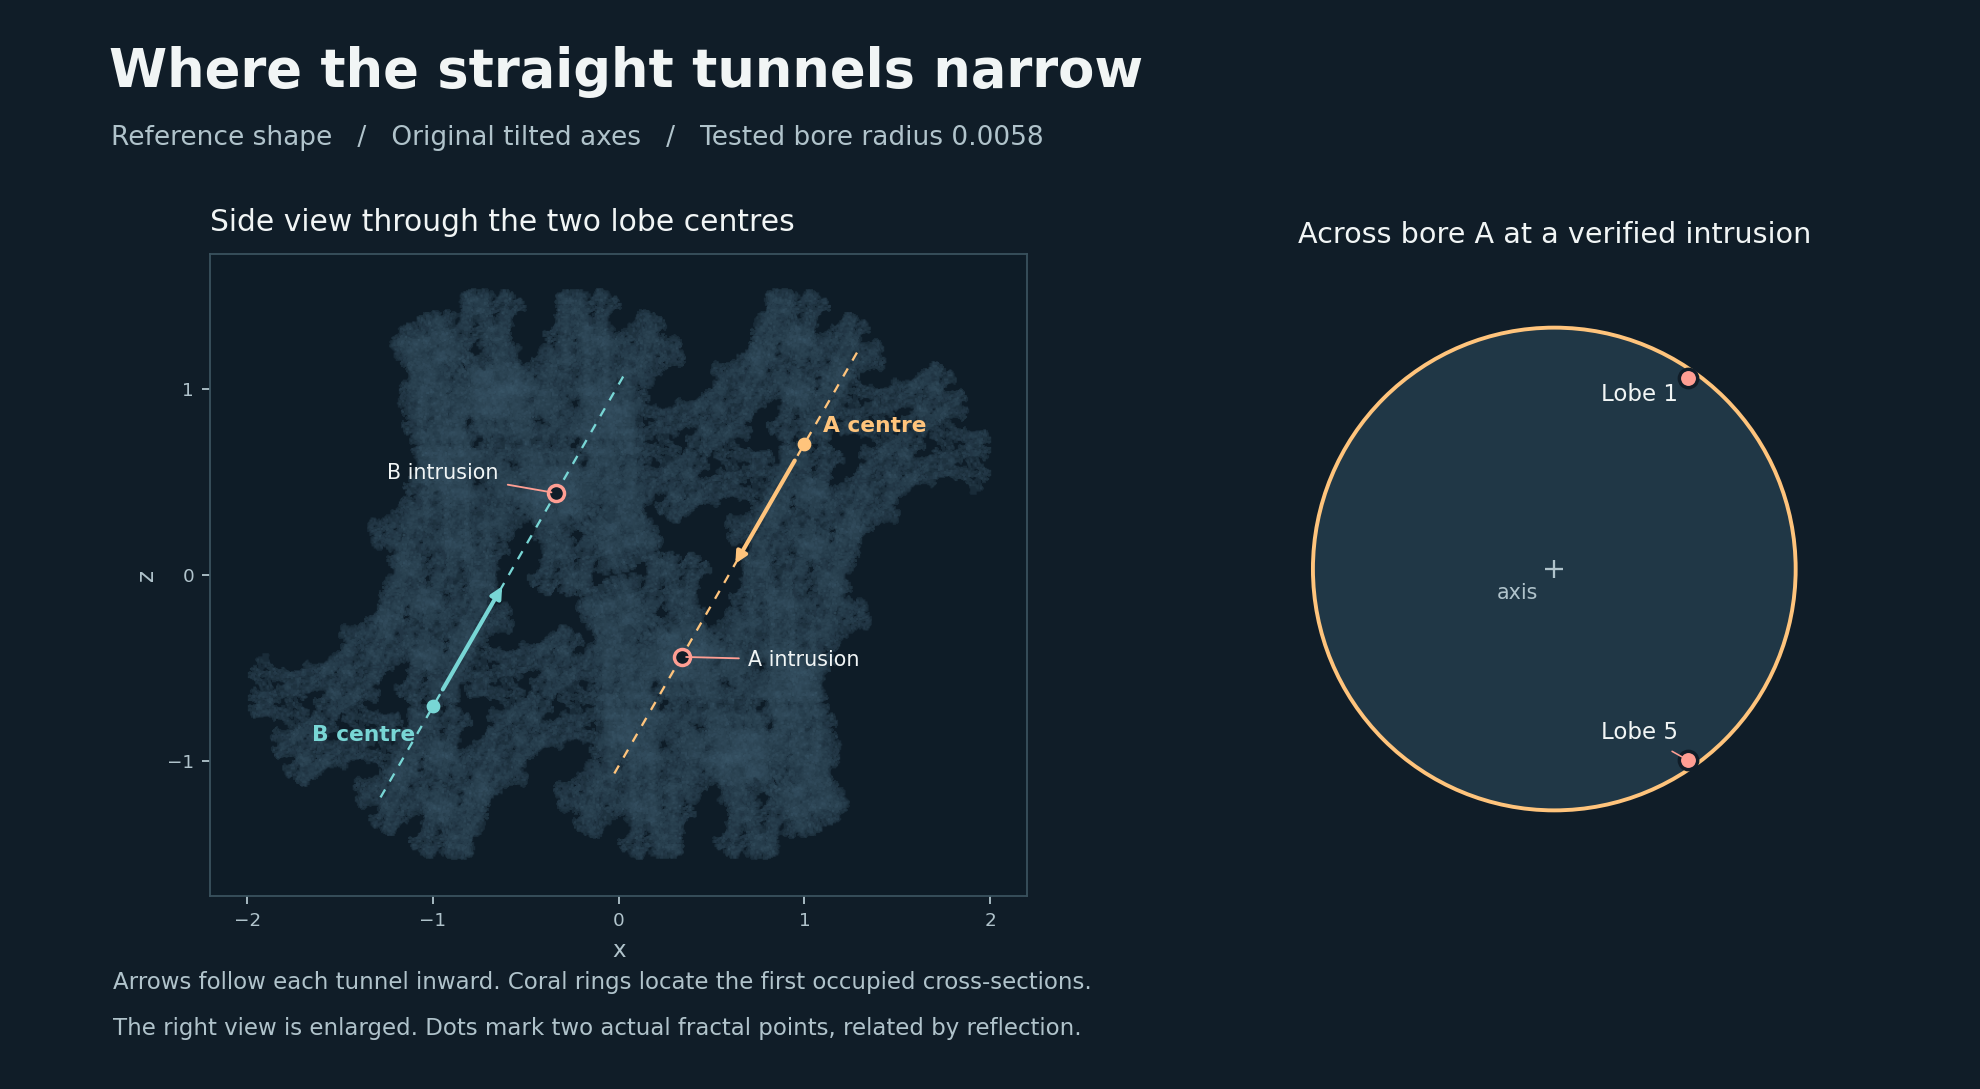
\includegraphics[width=\linewidth]{../research/fractal_research_10_topology/straight_axis_locator.png}
\caption{Obstruction of the inherited tilted bores at radius $0.0058$.
The enlarged cross-section marks actual addressed fractal points in lobes
1 and 5. Occupation of a positive-radius bore does not establish an exact
intersection with its centreline.}
\label{fig:bore}
\end{figure}

Whether the zero-width inherited axis meets $K$ remains open. Extremely close
addressed points and surviving branches of a finite search do not prove an
exact hit. The clear lines~\eqref{eq:axes} and Theorem~\ref{thm:homology} do
not depend on resolving this question. Here a ``tunnel'' denotes a certified
passage in the complement accompanied by a detected loop; it does not assume
a smooth wall or a solid body with a well-defined genus.
